% !TEX root = ../mechrelab.tex
\chapter{Orientation}\label{expt:01-lab-equp}

This is an introductory lab to get you oriented to the course's lab component, the equipment in the instrumentation lab, and learning to prototype simple electrical circuits with passive components in a breadboard. 

The logistics for the lab component of the course will be provided by the instructor at the start of the session. This will be followed by the course TAs and the instructor demonstrating the use of the equipment in the lab.

You will be required to build the following circuits and answer the questions associated with each circuit. You will be required to prepare a report on the circuits and the answers to the questions within a week of the lab session.

\section{Circuit 01: Series RC}
Build the following series RC circuit (Figure~\ref{fig:expt01-01}) on a breadboard and answer the following question:
\begin{figure}[htbp]
    \centering
    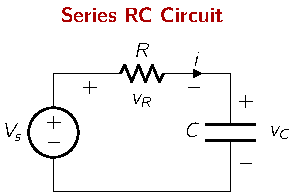
\includegraphics[width=0.5\textwidth]{figures/expt01/expt01-01.pdf}
    \caption{A series RC circuit.}
    \label{fig:expt01-01}
\end{figure}
\begin{enumerate}
    \item Propose a procedure for estimating the time constant for this circuit. You are free to choose any input signal $V_s$, but you must justify your choice. Based on this procedure, make your measurement, tabulate them, and estimate the time constant $\tau$ of the circuit. How does this value compare to the theoretical value of $\tau = RC$?
    \item Can you use this circuit or one with the appropriate modification to measure the input resistance of the oscilloscope? If so, how would you do it? Explain your procedure and estimate the input resistance of the oscilloscope.
\end{enumerate}

\section{Circuit 02: Parallel RC}
Build the following parallel RC circuit (Figure~\ref{fig:expt01-02}) on a breadboard and answer the following question:
\begin{figure}[htbp]
    \centering
    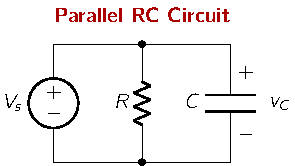
\includegraphics[width=0.5\textwidth]{figures/expt01/expt01-02.pdf}
    \caption{A parallel RC circuit.}
    \label{fig:expt01-02}
\end{figure}
\begin{enumerate}
    \item Derive the expression for the time constant $\tau$ for this circuit. You are free to choose any input signal $V_s$, but you must justify your choice. Based on this procedure, make your measurement, tabulate them, and estimate the time constant $\tau$ of the circuit. How does this value compare to the theoretical value of $\tau = RC$?
\end{enumerate}

\section{Circuit 03: RLC}
Let's now look at a more complex circuit, the parallel RLC circuit shown in Figure~\ref{fig:expt01-03}. Build this circuit on a breadboard and answer the following question, for $V_s = 5V$ (DC). Choose $R_s = 100\Omega$, which is used to limit the current drawn $V_s$.
\begin{enumerate}
    \item First, choose the value of the resistor to be $R = 1M\Omega$. Close the switch for some time, while measuring the voltage across $R$. What is the voltage across $R$ when the switch is closed for a long time?
    \item What happens when the switch is opened? Can you explain this behavior?
    \item Repeat the same experiment with $R=1k\Omega$. Is there any difference in the behavior of the circuit? If so, explain why.
    \item What is the frequency of oscillation of the circuit? How does it compare to the theoretical value of $f = \frac{1}{2\pi\sqrt{LC}}$?
\end{enumerate}
\begin{figure}[htbp]
    \centering
    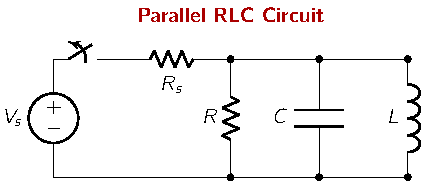
\includegraphics[width=0.75\textwidth]{figures/expt01/expt01-03.pdf}
    \caption{A parallel RLC circuit.}
    \label{fig:expt01-03}
\end{figure}

\section{Circuit 04: RC Circuit Sinusoidal Response}
In Figure~\ref{fig:expt01-01}, use a sinusoidal input for $V_s$ with amplitude $5V$. 
\begin{itemize}
    \item When you apply an input signal $V_s$ of any frequency, what is the frequency of the voltage across the capacitor? Is it the same or different?
    \item For an input of fixed amplitude, what happens to the amplitude of the voltage across the capacitor as the frequency of the input signal is varied? Tabulate your measurements of the output voltage amplitude across the capacitor for different input frequencies (0Hz to 1MHz). Plot the amplitude versus frequency.
    \item What is the phase difference between the input voltage and the voltage across the capacitor? How does this change with frequency?
\end{itemize}
Compare the results with the theoretical predictions for the circuit by doing the steady state sinusoidal analysis by using the impedance of the resistor and the capacitor.

\section{Circuit 05: RL Circuit Sinusoidal Response}
In Figure~\ref{fig:expt01-02}, use a sinusoidal input for $V_s$ with amplitude $5V$. 
\begin{itemize}
    \item When you apply an input signal $V_s$ of any frequency, what is the frequency of the voltage across the inductor? Is it the same or different?
    \item For an input of fixed amplitude, what happens to the amplitude of the voltage across the inductor as the frequency of the input signal is varied? Tabulate your measurements of the output voltage amplitude across the inductor for different input frequencies (0Hz to 1MHz). Plot the amplitude versus frequency.
    \item What is the phase difference between the input voltage and the voltage across the inductor? How does this change with frequency?
\end{itemize}
Compare the results with the theoretical predictions for the circuit by doing the steady state sinusoidal analysis by using the impedance of the resistor and the inductor.

\section{Circuit 06: Series RLC Circuit Sinusoidal Response}
In Figure~\ref{fig:expt01-04}, use a sinusoidal input for $V_s$ with amplitude $5V$. 
\begin{itemize}
    \item For an input of fixed amplitude, what happens to the amplitude of the voltage across the inductor as the frequency of the input signal is varied? Tabulate your measurements of the output voltage amplitude across the inductor for different input frequencies (0Hz to 1MHz). Plot the amplitude versus frequency.
    \item What is the phase difference between the input voltage and the voltage across the inductor? How does this change with frequency?
\end{itemize}
\begin{figure}[htbp]
    \centering
    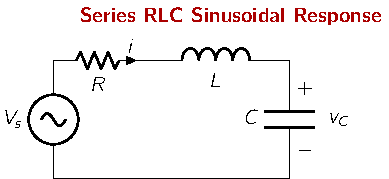
\includegraphics[width=0.75\textwidth]{figures/expt01/expt01-04.pdf}
    \caption{A series RLC circuit.}
    \label{fig:expt01-04}
\end{figure}
Compare the results with the theoretical predictions for the circuit by doing the steady state sinusoidal analysis by using the impedance of the resistor and the inductor.
